%%%%%%%%%%%%%%%%%%%%%%%%%%%%%%%%%%%%%%%%%%%%%%%%%%%%%%%%%%%%%%%%%%%%%%%%%%%%%%%%
\section{Lecture 4: Climate variability on a timescale of millions of years}

\subsection{Theory of plate tectonics}

\subsubsection{Alfred Wegener's hypothesis of continental drift}

\textbf{Glossopteris}: Example of a tree which is found fossilized (leaves)
on multiple continents.

\textbf{Caledonides}
The mountain chain in Scandinavia was once joined with Caledonides in
North-East America and North-West Africa. It was one mountain belt when all
continents were together.

\subsection{Patrick Blackett's polar wander}

If you look at volcanic rocks, as they solidify, they contain certain magnetic
minerals and they line up in magma as they crystallize, and they point towards
the North Pole.

\begin{figure}[H]
    \centering
    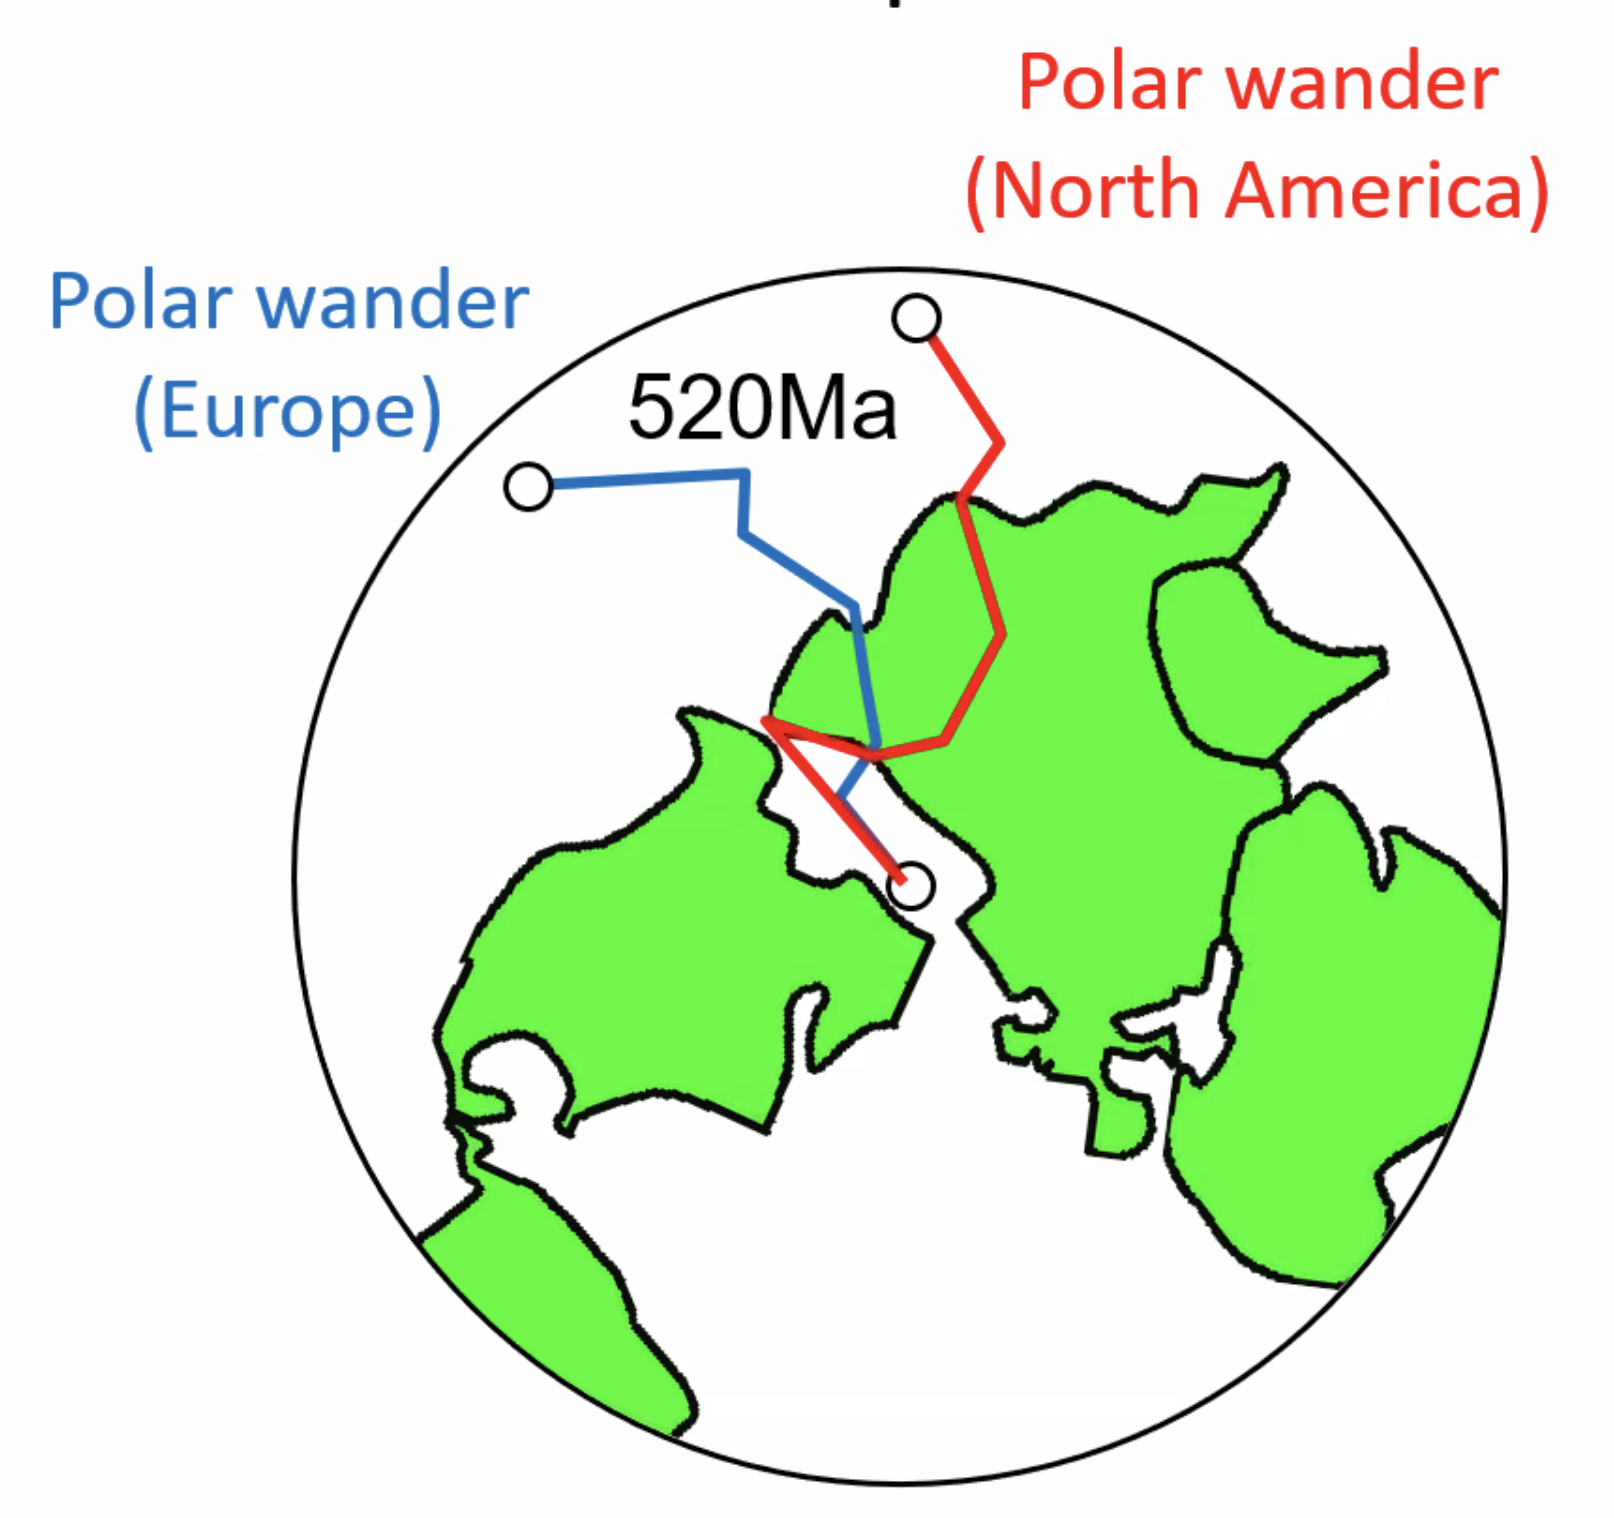
\includegraphics[width=0.5\linewidth]{content/img/polar_wander.png}
\end{figure}

\subsection{Ocean spreading}

Chicken and egg question: is the floor spreading because of volcanism, or is
the lava flowing because of spreading?

\begin{figure}[H]
    \centering
    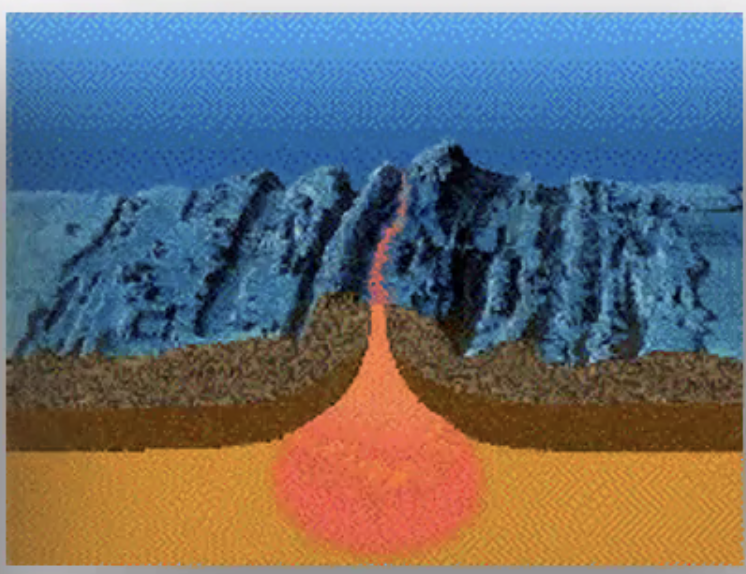
\includegraphics[width=0.5\linewidth]{content/img/ocean_floor_spreading.png}
\end{figure}

Ocean spreading increases CO$_2$ in the atmosphere (increased volcanism).
Mountain building does the opposite (more rocks for weathering).

\subsection{BLAG hypothesis}

\begin{figure}[H]
    \centering
    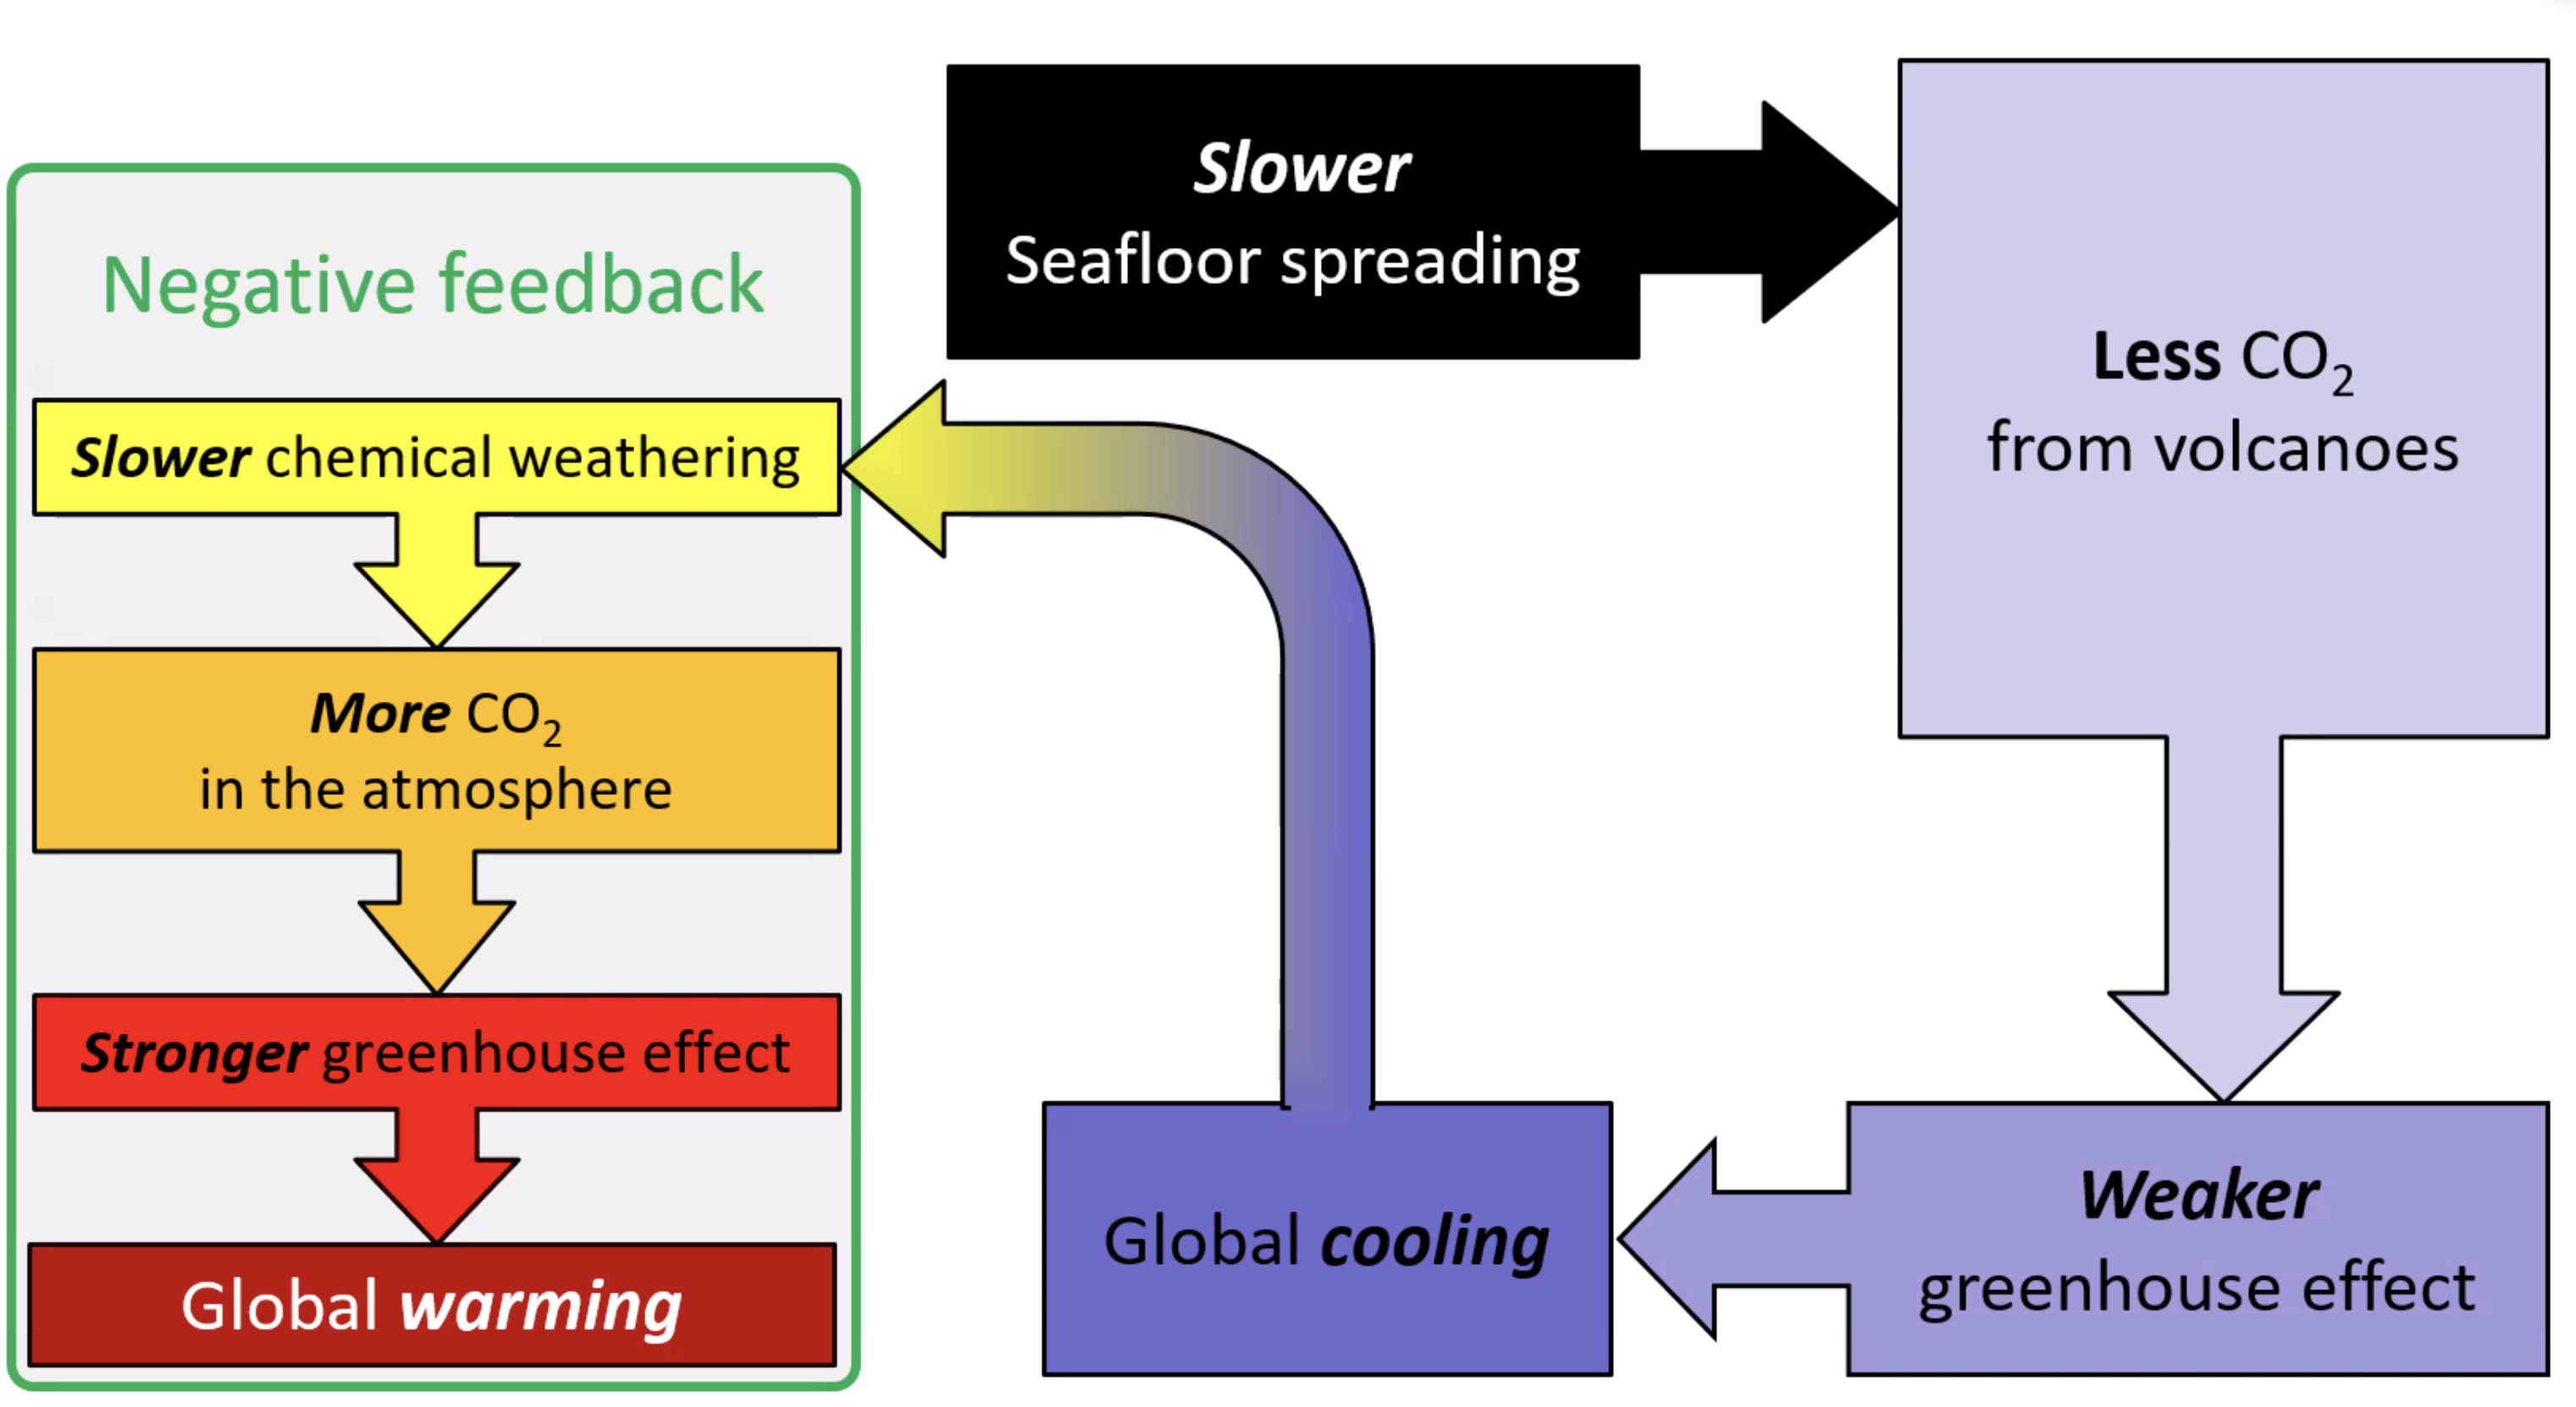
\includegraphics[width=\linewidth]{content/img/blag.png}
\end{figure}

\subsection{Uplift weathering hypothesis}

\begin{figure}[H]
    \centering
    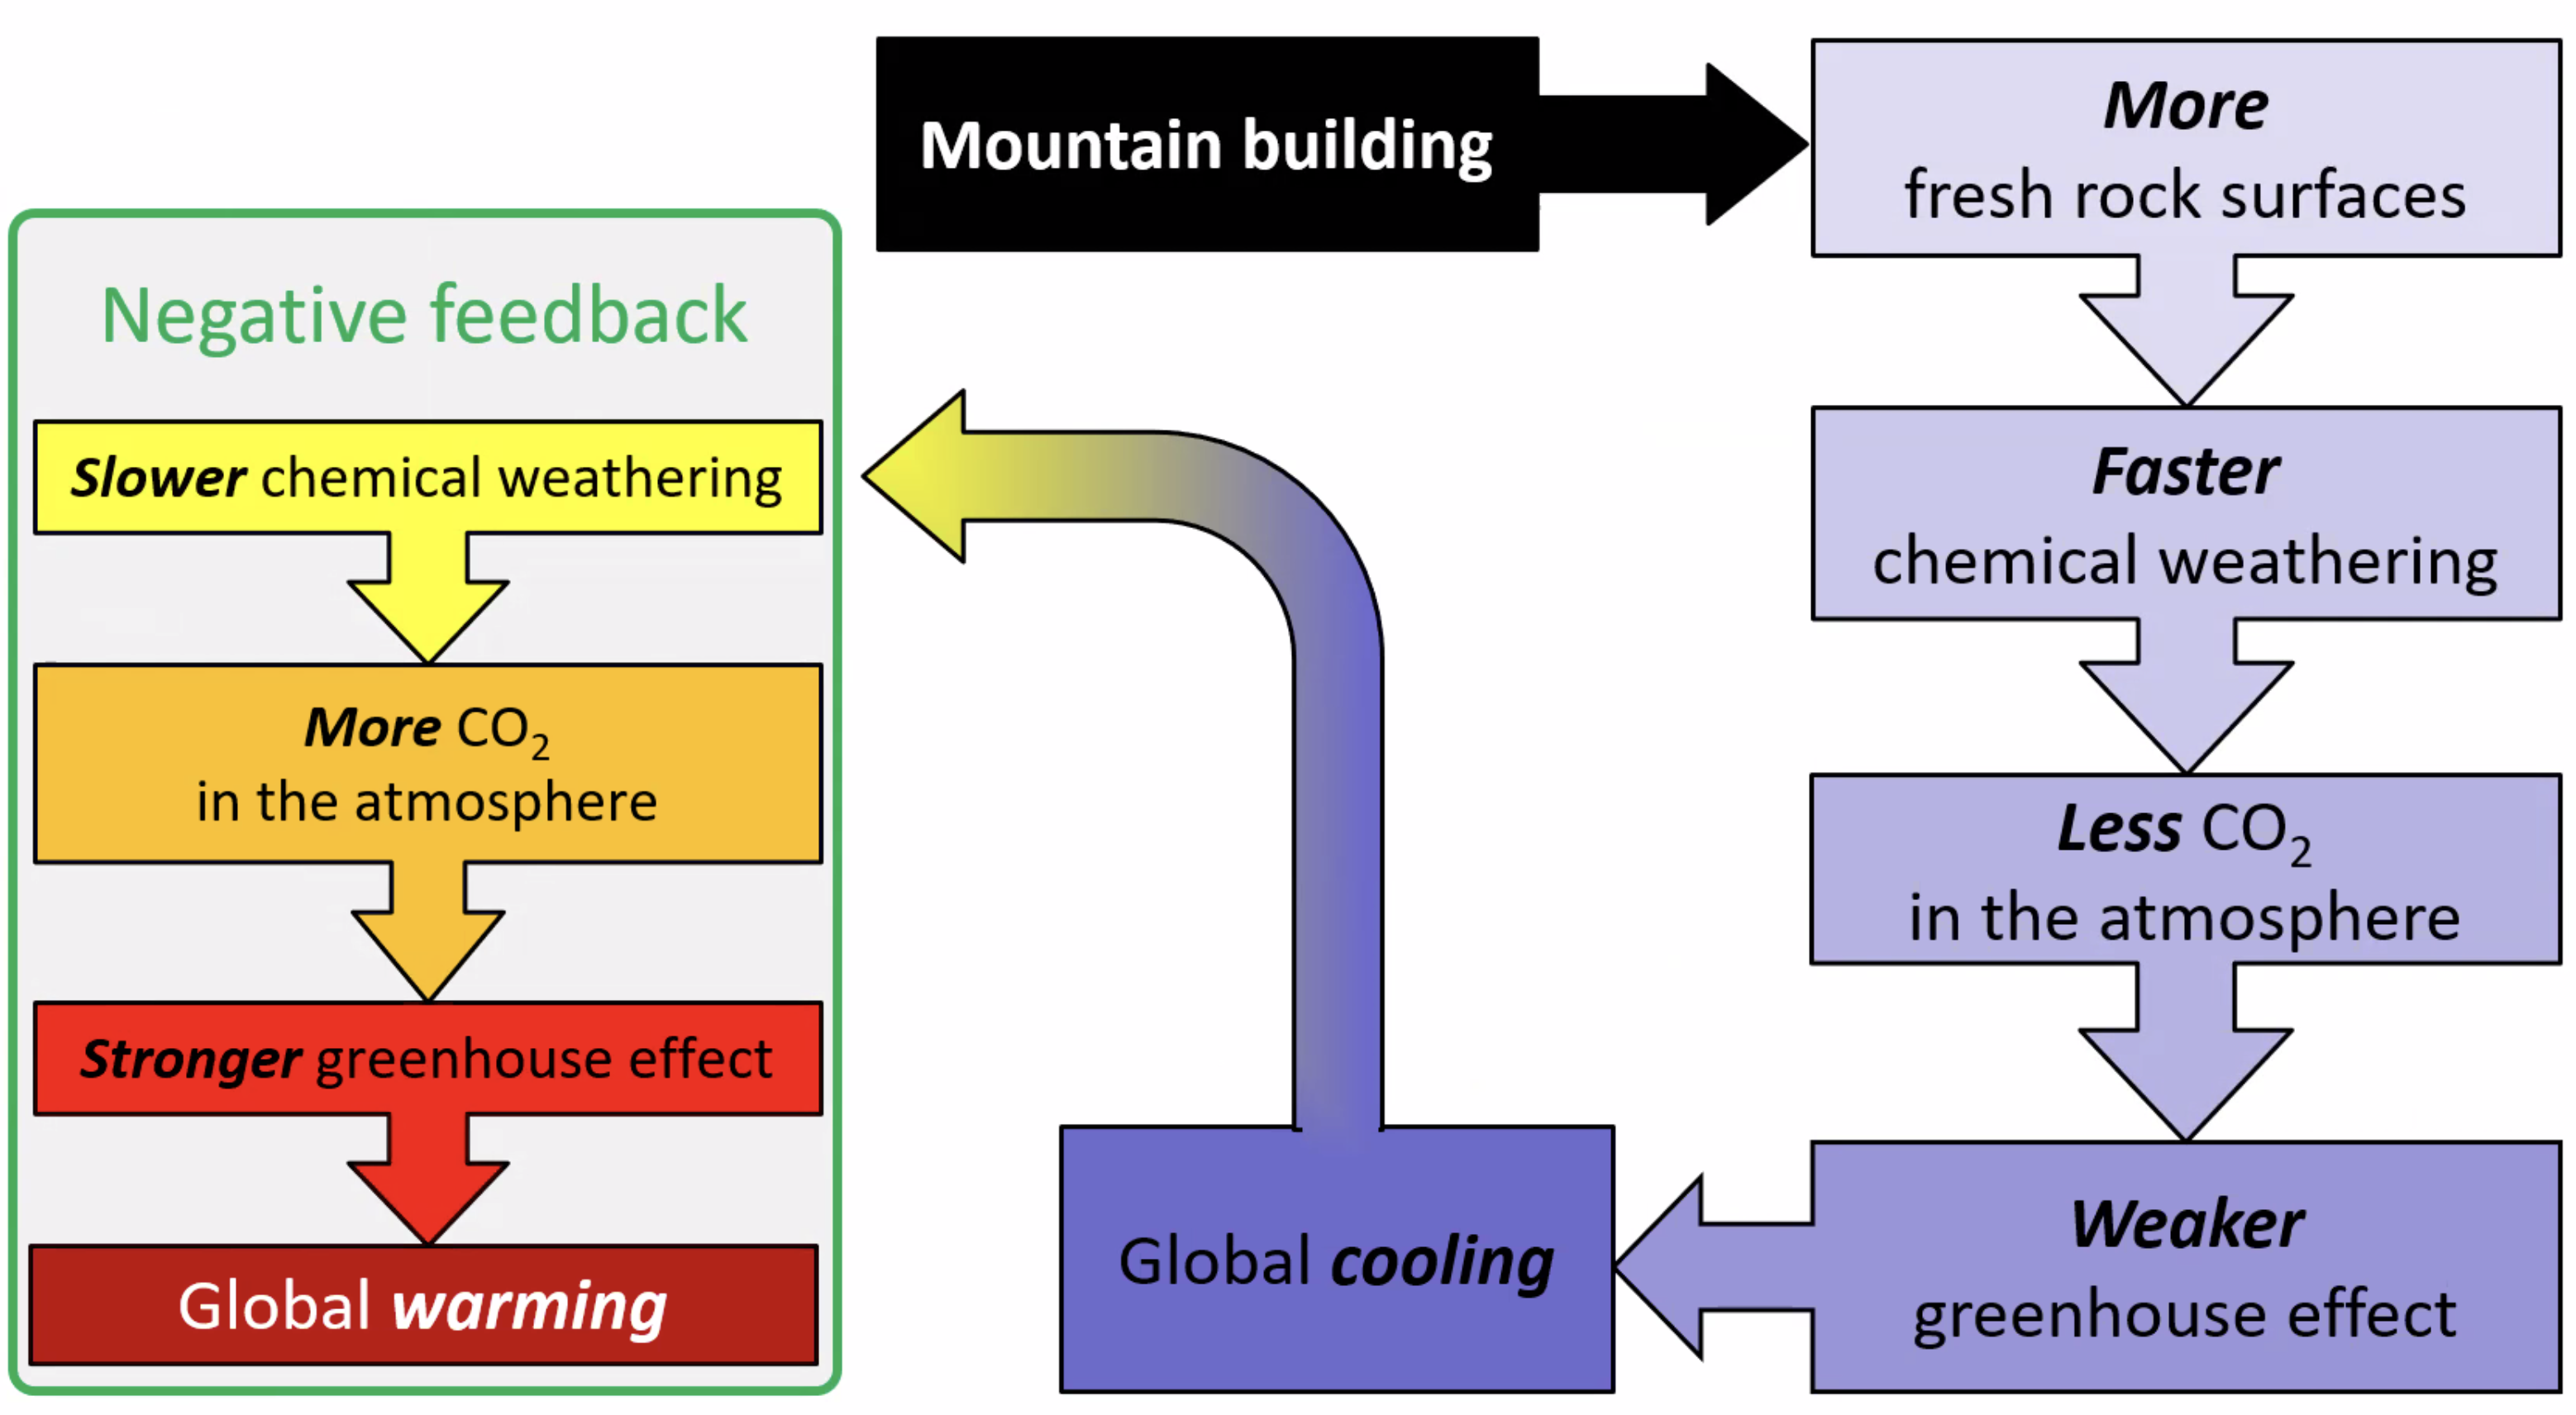
\includegraphics[width=1\linewidth]{content//img/uplift_weathering.png}
\end{figure}

\subsection{Polar position hypothesis}

Ice forms easier on land than on sea, which is the basis for polar position
hypothesis.

\begin{figure}[H]
    \centering
    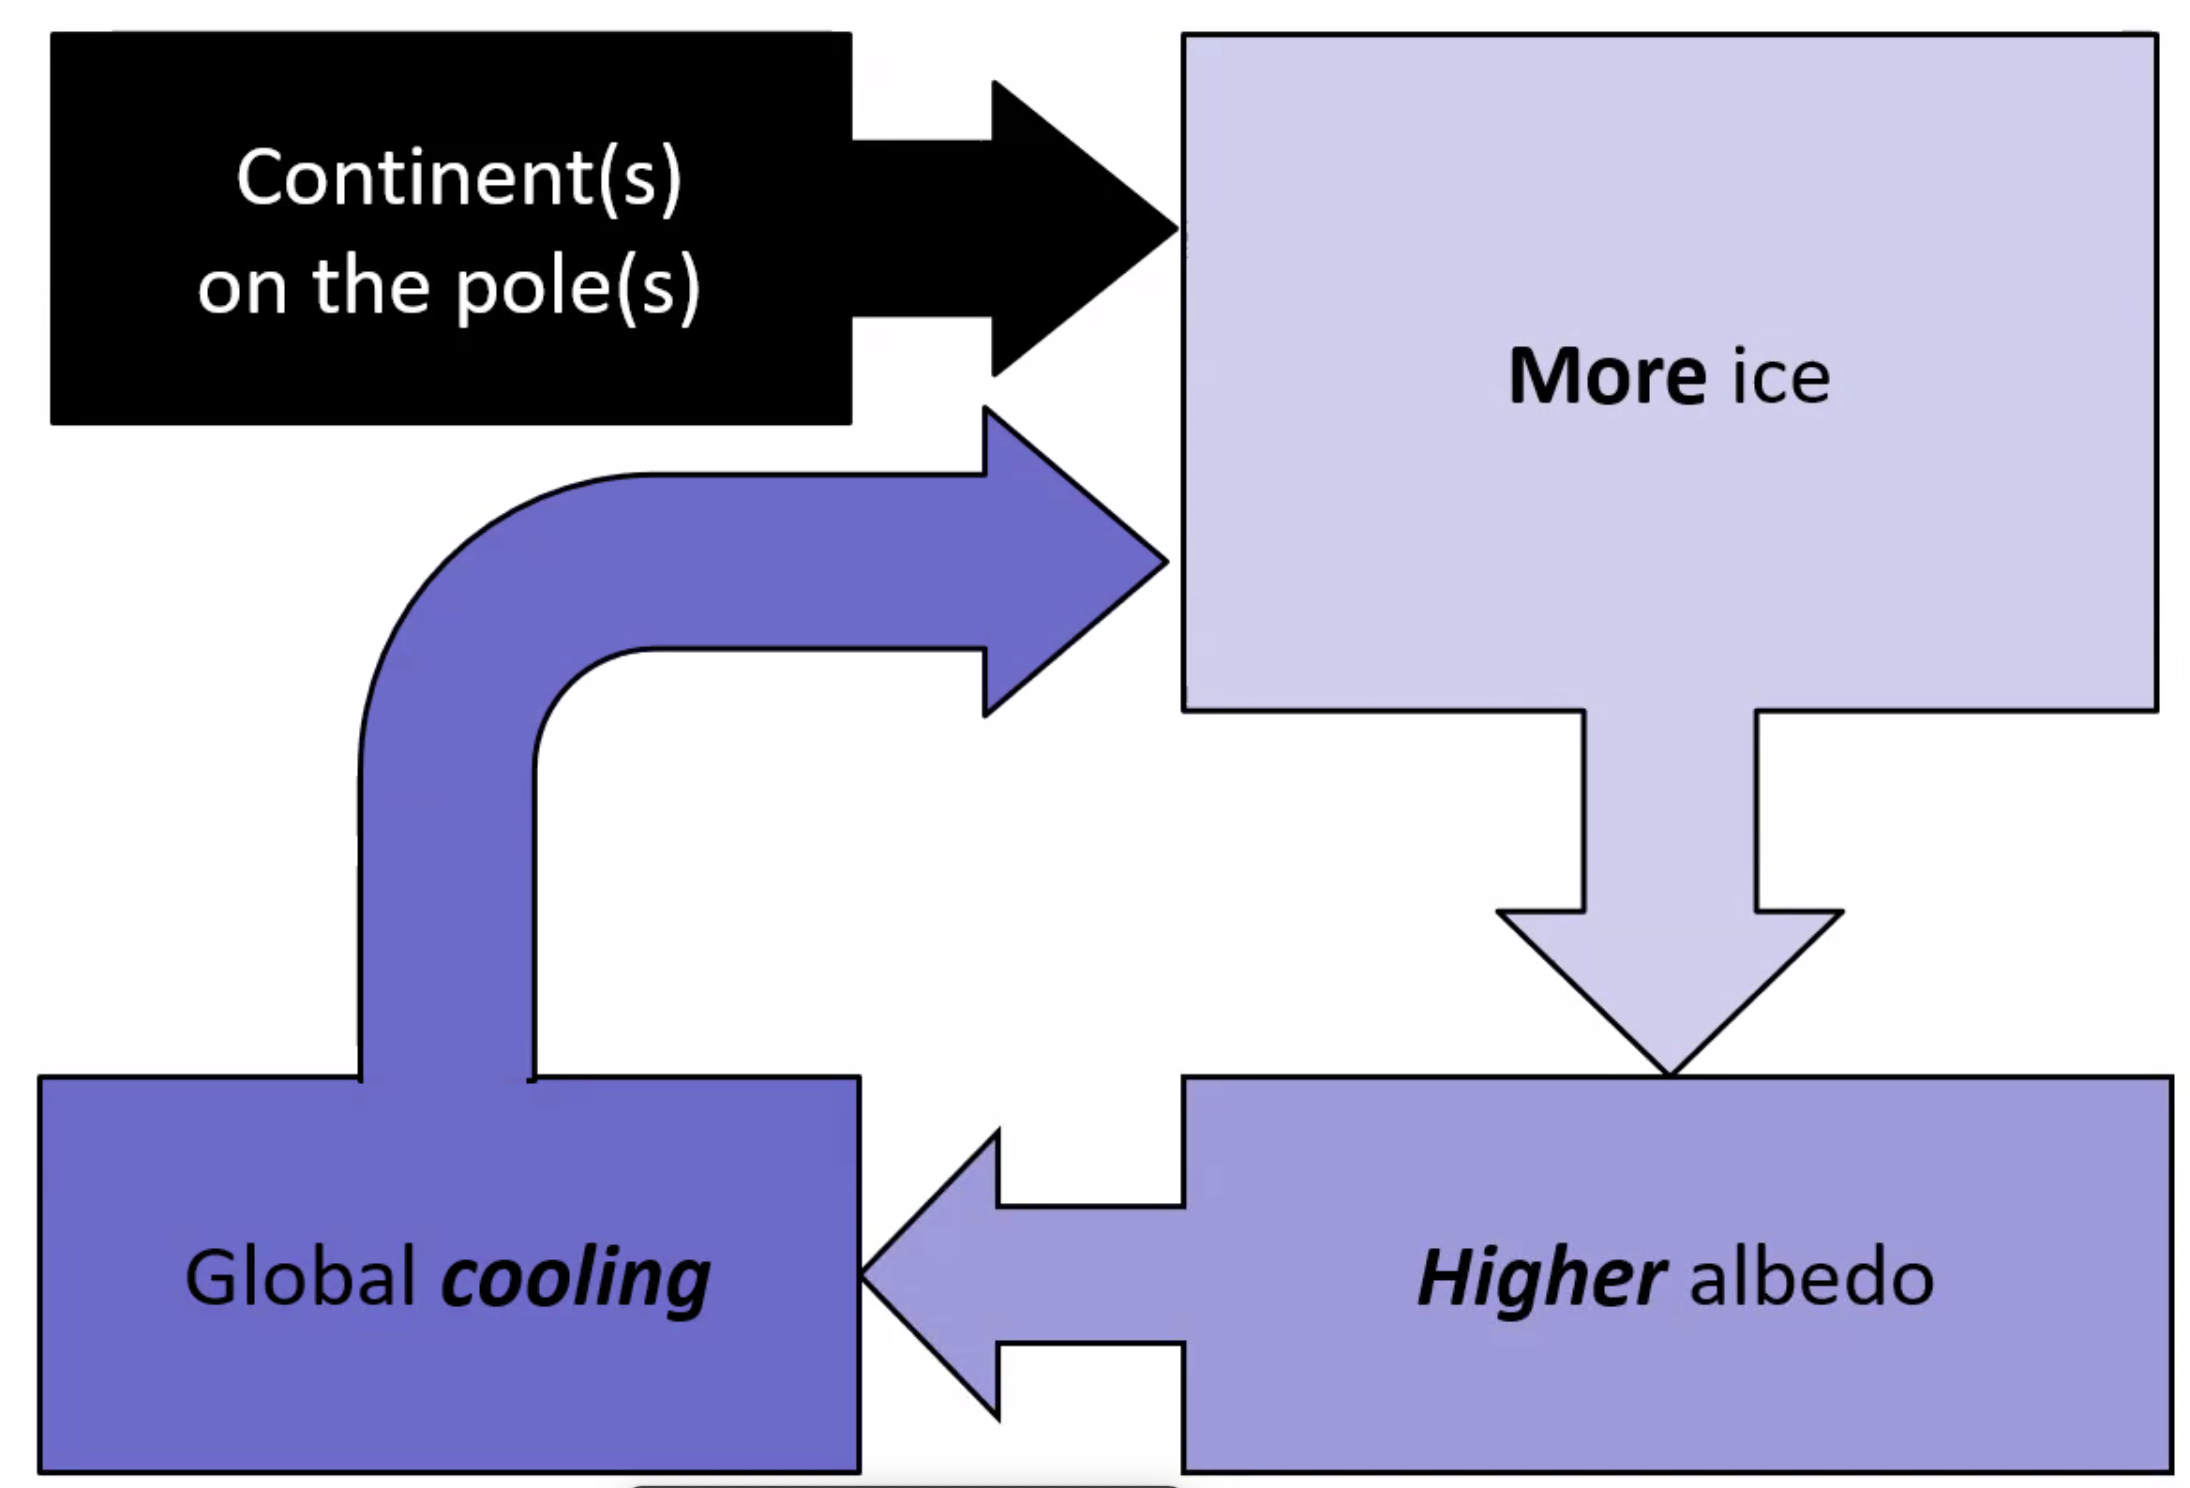
\includegraphics[width=1\linewidth]{
    content/img/polar_position_hypothesis.png}
\end{figure}

\subsection{Plate tectonics and climate}

\begin{itemize}
    \item \textbf{BLAG hypothesis}: slower seafloor spreading causes global
    cooling
    \item \textbf{Mountain building hypothesis}: mountain building causes
    global cooling
    \item \textbf{Polar position hypothesis}: land in polar positions causes
    global cooling
\end{itemize}

A continent (Antarctica) is on the South Pole, seafloor spreading is slow and
mountain building is ongoing forming the Himalaya. All these 3 suggest that the
climate should be cooling, not warming (when considering plate tectonics in
isolation).

%%%%%%%%%%%%%%%%%%%%%%%%%%%%%%%%%%%%%%%%%%%%%%%%%%%%%%%%%%%%%%%%%%%%%%%%%%%%%%%%